\chapter{\textit{Framework} PON C++
4.0}\label{ch:desenvolvimento}\label{sec:fw4_dev}

Esse capítulo apresenta os esforços realizados no desenvolvimento do
\textit{Framework} PON C++ 4.0. Primeiramente, na Seção \ref{sec:estrutura_fw4},
é apresentada de forma geral a estrutura do \textit{framework} em si, enquanto
as seções seguintes apresentam maiores detalhes de implementação de cada uma das
entidades do PON no \textit{framework}. A Seção \ref{sec:facilitadores}
também apresenta alguns conceitos introduzidos com o objetivo de facilitar o
desenvolvimento com o \textit{Framework} PON C++ 4.0. Ainda, a Seção
\ref{sec:unit_test} apresenta os testes desenvolvidos à luz do método
TDD. Por fim, a Seção \ref{sec:dev_reflex} reflete sobre os resultados
apresentados pelo desenvolvimento do \textit{Framework} PON C++ 4.0.

\section{Estrutura}\label{sec:estrutura_fw4}

A proposta do \textit{Framework} PON C++ 4.0 é solucionar de maneira suficiente
os problemas detalhados ao longo do Capítulo \ref{ch:arte}, como aqueles
reportados na Seção \ref{sec:problemas}, de acordo com os objetivos da Seção
\ref{sec:obj_especificos}. Para alcançar esses objetivos, propõe-se arquitetar
este novo \textit{framework}, nomeadamente \textit{Framework} PON C++ 4.0,
utilizando ferramentas de desenvolvimento de C++ dito moderno, como
\textit{smart pointers}, \textit{variadic templates}, \textit{fold expressions}
e expressões \textit{lambda}, fazendo a aplicação dos conceitos de programação
genérica e utilizando o método de desenvolvimento orientado a testes. 

Em resumo, a Tabela \ref{tab:obj_fw4} apresenta os principais objetivos a serem
atingidos com o desenvolvimento do \textit{Framework} PON C++ 4.0, à luz dos
objetivos da dissertação apresentados na Seção \ref{sec:obj_especificos}. Na
tabela são apresentados os problemas presentes nos \textit{frameworks}
anteriores e, de maneira sucinta, como o desenvolvimento do \textit{Framework}
PON C++ 4.0 pretende resolvê-los.

\begin{table}[!htb]
\centering
\caption{Problemas a serem endereçados pelo \textit{Framework} PON C++ 4.0}
\smallskip
\begin{tabularx}{\textwidth}{|l|X|}\hline
    Objetivo & Proposta   \\\hline\hline
    Adicionar a flexibilidade de tipos & \textit{Attribute} com tipo \textit{template} \\ \hline
    Adicionar flexibilidade algorítmica & \textit{Condition} com expressões \textit{lambda} \\ \hline
    Reduzir a verbosidade da utilização & \textit{Builders} com \textit{variadic templates} \\ \hline
    Permitir execução com paralelismo & Notificações com políticas de execução \\ \hline
\end{tabularx}
\caption*{Fonte: Autoria própria}
\label{tab:obj_fw4}
\end{table}

Em tempo, naturalmente trechos de código do proposto \textit{Framework} PON C++
4.0 serão apresentados ao longo deste capítulo, de forma a explicar avanços e
melhorias nele. Entretanto, para fins de simplicidade, os trechos de código em
sua maior parte omitem alguns detalhes de implementação, apresentando apenas os
trechos necessários para a compreensão dos conceitos de forma
adequada\footnote{O código completo do \textit{Framework} PON C++ 4.0 atualizado
também pode ser consultado no servidor de artefatos do PON, uma vez que se tenha
acesso a ele (via login e senha) em
\url{https://nop.dainf.ct.utfpr.edu.br/nop-implementations/frameworks/nop-framework-cpp-4}.}.
%Ainda, o
%código completo do \textit{Framework} PON C++ 4.0 pode ser consultado no
%\nameref{ap:fw_full}.

De forma a facilitar o entendimento dos conceitos e técnicas aplicados no
\textit{Framework} PON C++ 4.0 e apresentados ao longo deste capítulo, será
utilizado o exemplo da aplicação de sensores, que também já foi introduzido na
Figura \ref{fig:nop_rule} da Seção \ref{sec:pon}. A representação deste
\textit{FBE} e \textit{Rule} em NOPL e sua implementação com o
\textit{Framework} PON C++ 4.0 são apresentados, no Código \ref{cod:fw4_sensor}.
Nestes exemplos destaca-se que,
salvo as peculiaridades da linguagem de programação C++ (como inicialização das
variáveis), ambos os exemplos apresentam estruturas bastante
similares\footnote{Existe compilador de NOPL para \textit{Framework} PON C++
4.0 desenvolvido por \citeonline{skora_2020}}.

\begin{lstlisting}[language=C++, float=htb,
    caption = {Implementação do \textit{FBE} \textit{Sensor} em \textit{Framework} PON C++ 4.0},
    source = {Autoria própria},
    label = {cod:fw4_sensor}]
/*
fbe Sensor
    public boolean atIsRead = false
    public boolean atIsActivated = false
    private method mtProcess
        attribution
            this.atIsRead = true
            this.atIsActivated = false
        end_attribution
    end_method
    rule rlSensor
        condition
            premise prIsActivated
            this.atIsActivated == true
            end_premise
            and
            premise prIsNotRead
            this.atIsRead == false
            end_premise
        end_condition
        action sequential
            instigation sequential
            call this.mtProcess()
            end_instigation
        end_action
    end_rule
end_fbe
*/
struct NOPSensor: NOP::FBE {
    // Essa é a parte relativa a definição do FBE
    // Aqui se declaram e inicializam os Attributes
    NOP::SharedAttribute<bool> atIsRead{NOP::BuildAttribute(false)};
    NOP::SharedAttribute<bool> atIsActivated{NOP::BuildAttribute(false)};
    // Aqui se define o Method utilizando uma expressão lambda
    NOP::Method mtProcess{[&]()(
            atIsRead->SetValue(true);
            atIsActivated->SetValue(false);
        )};
    // Essa é a parte relativa a definição da Rule agregada ao FBE
    // com a definição das respectivas Premises, Condition, Action
    // e Instigation que a compõe
    NOP::SharedRule rlSensor{NOP::BuildRule(
        NOP::BuildCondition<NOP::Conjunction>( 
            NOP::BuildPremise(atIsActivated, true, NOP::Equal()), 
            NOP::BuildPremise(atIsRead, false, NOP::Equal())
            ),
        NOP::BuildAction(
            NOP::BuildInstigation(mtProcess)
            )
        )
    };
};
\end{lstlisting}

Isto dito, o já bem supra salientado precedente \textit{Framework} PON C++ 2.0
foi construído com base no C++98, que contém um conjunto de recursos muito
limitado quando comparado às versões mais novas disponíveis, como C++20. De
maneira geral, a despeito da implementação em si, o modelo/projeto de estrutura
de classes em UML em si do pacote \textit{Core} do \textit{Framework} PON C++
2.0, apresentado na Figura \ref{fig:class_fw2_core}, segue pertinente. Assim, a
implementação \textit{Framework} PON C++ 4.0 naturalmente apresenta uma
modelagem inspirada no modelo de estrutura de classes similar ao do
\textit{Framework} PON C++ 2.0, porém naturalmente faz algumas simplificações,
visando aumentar a facilidade de uso do código decorrente.

\begin{figure}[!htb]
    \centering
    \caption{Diagrama de classes do pacote \textit{Core} do \textit{Framework}
        PON C++ 2.0} 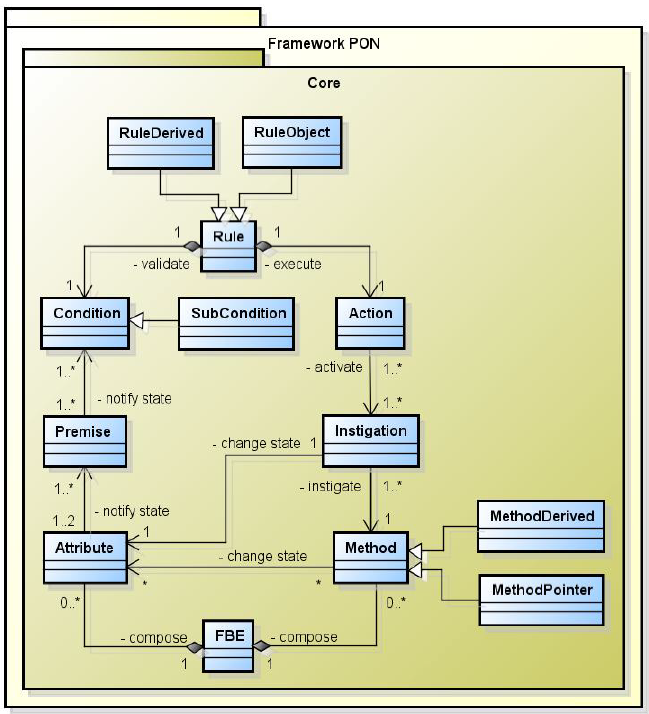
\includegraphics[width=0.7\textwidth]{../figures/fw2_core.PNG}
    \smallskip
    \caption*{Fonte: \citeonline{msc_Ronszcka_2012}}
    \label{fig:class_fw2_core}
\end{figure}


%\footnote{C++20 é a versão mais recente com suporte disponível nos
%principais compiladores durante o desenvolvimento deste projeto}

O diagrama de classes para modelagem do \textit{Framework} PON C++ 4.0, por sua
vez, é apresentado na Figura \ref{fig:class_fw4}. Nesse contexto, podem
ser destacadas as principais diferenças entre as duas versões, sendo a principal
diferença a eliminação do pacote \textit{Application}, detalhado anteriormente
na Figura \ref{fig:fw2_struct}. Isto é viabilizado ao utilizar elementos
mais desacoplados que não precisam de estruturas gerenciadoras acoplantes.

O \textit{Framework} PON C++ 4.0, ao adotar uma estrutura mais genérica, elimina
a necessidade da implementação de classes especializadas e potencialmente
redundantes (\textit{e.g.}, \textit{MethodDerived}, \textit{MethodPointer},
\textit{RuleObject}, \textit{RuleDerived} e \textit{SubCondition}). No lugar da
\textit{SubCondition}, de modo a alcançar a mesma funcionalidade sem se tornar
necessária uma especialização da classe, foi implementada uma agregação entre as
próprias \textit{Conditions}.

\begin{figure}[!htb]
    \centering
    \caption{Diagrama de classes do \textit{Framework} PON C++ 4.0}
    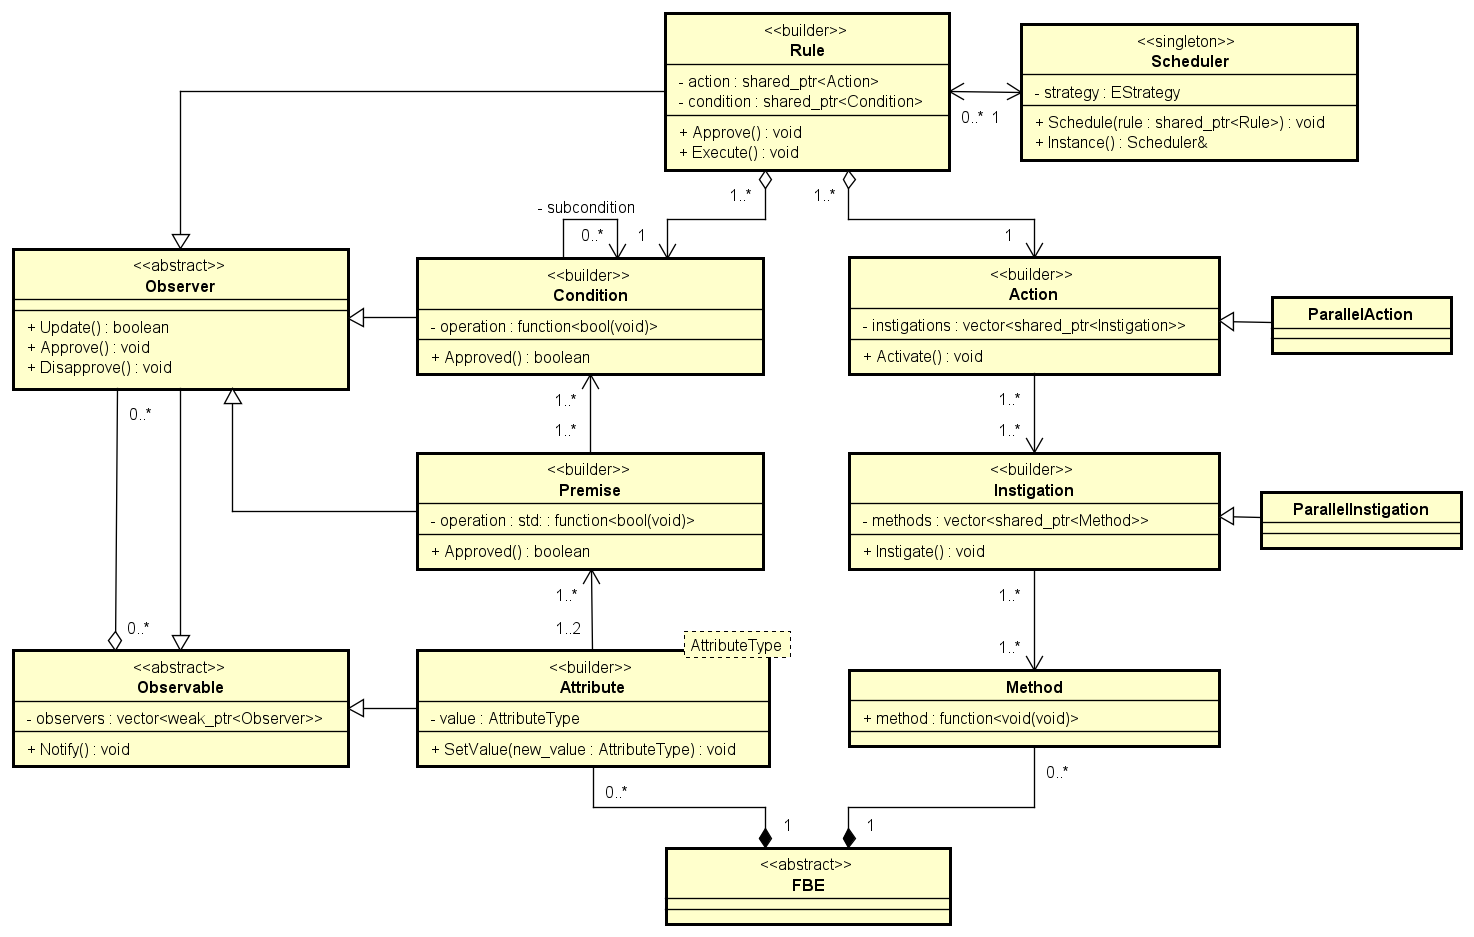
\includegraphics[width=\textwidth]{../figures/astah_nop4.png}
    \smallskip
    \caption*{Fonte: Autoria própria}
    \label{fig:class_fw4}
\end{figure}

\FloatBarrier

A implementação também contempla a utilização de um escalonador de
\textit{Rules}, que pode ser utilizado para controlar o fluxo de execução das
\textit{Rules} aprovadas. Esse escalonador é materializado pela classe
\textit{Scheduler}, que usa o padrão de projeto \textit{Singleton},
implementando as estratégias de escalonamento de \textit{Rules} equivalentes às
propostas por \citeonline{msc_Banaszewski_2009} (\textit{Breadth},
\textit{Depth}, \textit{Priority}, \textit{NoOne}, detalhadas na Seção
\ref{sec:conflitos}) e reaplicadas por \citeonline{msc_valenca_2012} e
\citeonline{msc_Ronszcka_2012}.

A classe \textit{Premise}, apesar de se associar a \textit{Attributes} com tipos
\textit{template}, não utiliza \textit{template}. Isso se torna possível por
essa associação ser realizada por meio da utilização de expressões
\textit{lambda}, que permitem abstrair o tipo dos \textit{Attributes} sobre o
qual a \textit{Premise} opera, interessando a essa apenas o tipo de retorno da
expressão de comparação dos \textit{Attributes}, que no caso será sempre um tipo
\textit{bool}.

Por fim, do ponto de vista de padrão de projetos, aproveitam-se os conceitos
introduzidos por \citeonline{msc_Ronszcka_2012}, sendo que no \textit{Framework}
PON C++ 4.0 são utilizados os padrões \textit{Observer}, \textit{Iterator},
\textit{Builder} e \textit{Singleton}. A Tabela \ref{tab:padroes} sumariza onde
cada padrão é aplicado no \textit{framework}, enquanto detalhes sobre os padrões
de projeto em si são discutidos ao longo do capítulo.

Dada esta introdução sobre a estrutura do \textit{Framework} PON C++ 4.0, as
seções seguintes se encarregam de detalhar a implementação de cada um de seus
componentes, inclusive da implementação de cada uma das entidades do PON.
Utiliza-se neste capítulo uma abordagem \textit{bottom-up}, ou seja, parte-se da
explicação do cerne do \textit{framework}, dado pelo mecanismo de notificações,
seguido das entidades principais, e por fim as abstrações e facilitadores de
desenvolvimento.

\begin{table}[!htb]
    \centering
    \caption{Padrões de projeto aplicados no \textit{Framework} PON C++ 4.0}
    \smallskip
    \begin{tabularx}{\textwidth}{|l|X|}\hline
        Padrão de projeto & Aplicação   \\\hline\hline
        \textit{Observer} & Aplicado para a implementação do mecanismo de notificações \\ \hline%, conforme apresentado na Seção \ref{sec:observer} \\ \hline
        \textit{Iterator} & Utilizado por meio dos \textit{iterators} da STL na estrutura de dados \textit{std::vector} \\ \hline
        \textit{Builder} & Aplicado para a implementação dos construtores das entidades do PON \\ \hline%, conforme apresentado na Seção \ref{sec:builders} \\ \hline
        \textit{Singleton} & Aplicado para a implementação do escalonador de
        \textit{Rules} \\ \hline%, conforme apresentado na Seção \ref{sec:scheduler}\\ \hline
    \end{tabularx}
    \caption*{Fonte: Autoria própria}
    \label{tab:padroes}
    \end{table}

\section{Mecanismo de notificações}\label{sec:observer}

O mecanismo de notificações faz parte do cerne do \textit{framework}, sendo
responsável por possibilitar as interações entre as entidades do PON, que
interagem entre si por meio de notificações pontuais. No \textit{Framework} PON
C++ 4.0, do mesmo modo que no \textit{Framework} PON C++ 2.0, optou-se por
utilizar o padrão de projeto \textit{Observer} para tal. O padrão de projeto
\textit{Observer} define uma relação de um para muitos entre objetos. Nesse
padrão, na mudança de estado de um objeto, todos os objetos interessados nesta
mudança são notificados \cite{gamma_1995,msc_Ronszcka_2012}.

A implementação do padrão de projeto \textit{Observer} no \textit{Framework} PON
C++ 4.0 é dada por meio das classes \textit{Observer} e \textit{Observable}.
Estas classes são utilizadas para materializar o mecanismo de notificações do
PON, e implementadas de modo a facilitar a reutilização de código e remover a
duplicidade de código no \textit{framework}. Tanto a classe \textit{Observer}
como \textit{Observable} são classes abstratas, servindo de modo a abstrair o
processo de notificações das classes \textit{Attribute}, \textit{Premise},
\textit{Condition} e \textit{Rule}. Isto foi preservado a partir do
\textit{Framework} PON C++ 2.0, ajustando para o contexto do \textit{Framework}
PON C++ 4.0.

Em detalhe no Código \ref{cod:observer_h}, a classe \textit{Observer} possui um
método \textit{Update} que permite a instância de classes derivadas notificar
algum estado pertinente. O método \textit{Update} é chamado por instância da
classe \textit{Observable} quando ela deseja notificar. Ainda na classe
\textit{Observer} há o método virtual \textit{Approve} que pode ser
especializado pelas classes para realizar tratamentos específicos em caso de
aprovação, como o caso da \textit{Rule} que deve executar a sua \textit{Action},
enquanto para outras entidades (\textit{i.e.}, \textit{Attribute},
\textit{Premise}, \textit{Condition}) ele não precisa ser especializado. 
%Além disso, ambas as classes \textit{Action} e \textit{Instigation} possuem uma
%especialização para fins de implementação paralelizada, por meio das classes
%\textit{ParallelAction} e \textit{ParallelInstigation}.

Já a classe \textit{Observable}, em destaque no Código \ref{cod:observable_h},
possui apenas 2 métodos, \textit{Attach} que permite a instâncias adicionar um
novo \textit{Observer} a sua lista de entidades a serem notificadas, e
\textit{Notify} que permite a tais instâncias realizar as notificações de fato.
Para o armazenamento das entidades é declarada a estrutura genérica
\textit{NOPContainer}, que pode ser especializada de modo a utilizar qualquer
estrutura de dado sem necessitar de alterações no código. A classe
\textit{Observer} também deriva de \textit{std::shared\_from\_this}, que é uma
classe da STL utilizada para permitir de forma simples acessar um
\textit{shared\_ptr} em funções membros da própria classe, de forma análoga ao
uso de \textit{raw pointers} que são acessíveis por meio do ponteiro
\textit{this}.

\begin{lstlisting}[language=C++, float=htb,
caption = {Implementação da classe \textit{Observer} no \textit{Framework} PON C++ 4.0},
source = {Autoria própria},
label = {cod:observer_h}]
class Observer : public Observable
{
   public:
    virtual bool Approved() = 0;
    template <NOPFlag Flag = Default>
    bool Update();
    virtual void Approve();
    virtual void Disapprove();

   protected:
    bool approved_{false};
};
\end{lstlisting}


\begin{lstlisting}[language=C++, float=htb,
caption = {Implementação da classe \textit{Observable} no \textit{Framework} PON C++ 4.0},
source = {Autoria própria},
label = {cod:observable_h}]
class Observable
{
   public:
    void Attach(const std::shared_ptr<class Observer>& observer);
    template <NOPFlag Flag = Default>
    void Notify();

   private:
    NOPContainer<std::weak_ptr<class Observer>> observers_;
};
\end{lstlisting}
\FloatBarrier

No \textit{Framework} PON C++ 4.0 a estrutura \textit{NOPContainer} utiliza
\textit{std::vector} da STL, não sendo implementada uma estrutura de dados
própria, simplemente definindo o template conforme apresentado no Código
\ref{cod:nopcontainer}. No \textit{Framework} PON C++ 4.0 optou-se pela
utilização apenas do tipo \textit{std::vector} ao invés da criação de estruturas
de dados otimizadas, como \textit{NOPLIST}, \textit{NOPVECTOR} e
\textit{NOPHASH} do \textit{Framework} PON C++ 2.0, pois \textit{std::vector}
pode ser facilmente utilizada com a aplicação de algoritmos paralelizados do
C++.

\begin{lstlisting}[language=C++, float=htb,
caption = {Definição de \textit{NOPContainer} no \textit{Framework} PON C++ 4.0},
source = {Autoria própria},
label = {cod:nopcontainer}]
template <typename T>
using NOPContainer = std::vector<T>;
\end{lstlisting}

Ainda assim, \textit{NOPContainer} pode ser implementado como qualquer estrutura
de dados compatível com as interfaces de uso da STL com \textit{std::vector},
com a capacidade de inserção e remoção de elementos, assim como a navegação por
iteradores. Entretanto, tal implementação adiciona significante grau de
complexidade, e potencialmente vulnerabilidades no contexto da aplicação
paralelizada. Nesse sentido, há uma troca de potencial ganho de desempenho por
maior garantia de estabilidade.

O processo de notificação em si acontece por meio da chamada do método
\textit{Notify} nas instâncias, que utiliza \textit{iterators} para navegar
entre todos os elementos do \textit{NOPContainer}, realizando a chamada do
método \textit{Update} da respectiva instância de \textit{Observer}. Por meio
do uso de \textit{templates} e expressões constantes, os diferentes métodos de
notificação podem ser implementados nessa mesma função sem acarretar custos
suplementares de desempenho em tempo de execução. Esse mecanismo é mostrado no
Código \ref{cod:observable_cpp}. Nesse código é interessante observar o uso
extensivo de expressões constantes, o que traz grandes benefícios em redução de
tempo de execução ao eliminar a execução de instruções condicionais, pelo fato
de ser um método muito utilizado, por meio da utilização de \textit{if
constexpr} com parâmetros de \textit{template}.

\begin{lstlisting}[language=C++,
caption = {Método \textit{Notify} da classe \textit{Observable} no \textit{Framework} PON C++ 4.0},
source = {Autoria própria}, float=htb,
label = {cod:observable_cpp}]
template <NOPFlag Flag>
inline void Observable::Notify()
{
    // Define expressão lambda para notificar entidades
    auto notify_entities = [](auto& observer)
    {
        bool ret{false};
        if (const auto& observer_ptr = observer.lock(); observer_ptr)
        {
            ret = observer_ptr->template Update<Flag>();
        }
        return ret;
    };

    if constexpr (0 < (NoNotify & Flag))
    {
        // Não notifica
    }
    else if constexpr (0 < (Parallel & Flag))
    {
        if constexpr (0 < (Exclusive & Flag))
        {
            // Notifica todas as entidades com execução de forma paralelizada 
            // até a o primeiro update retornar TRUE quando a entidade é aprovada
            const bool ret =
                std::none_of(std::execution::par_unseq, observers_.begin(),
                             observers_.end(), notify_entities);
        }
        else
        {
            // Notifica todas as entidades com execução
            // de forma paralelizada
            std::for_each(std::execution::par_unseq, observers_.begin(),
                          observers_.end(), notify_entities);
        }
    }
    else if constexpr (0 < (Exclusive & Flag))
    {
        // Notifica todas as entidades de forma sequencial até 
        // o primeiro update retornarTRUE quando a entidade é aprovada
        const bool ret =
            std::none_of(observers_.begin(), observers_.end(), notify_entities);
    }
    else
    {
        // Caso padrão
        // Notifica todas as entidades de forma sequencial
        std::for_each(observers_.begin(), observers_.end(), notify_entities);
    }
}
\end{lstlisting}

O método \textit{Update} utiliza o parâmetro \textit{Parallel} para determinar a
execução do mecanismo de notificações de forma paralelizada. Com isso, todas as
notificações geradas por determinada entidade são realizadas de forma
paralelizada. Cabe aqui detalhar que a paralelização é alcançada por meio da
aplicação de políticas de execução, evidentes pelo uso de
\textit{std::execution::par\_unseq}. Ainda, é importante reforçar que com o uso
da política de execução, o balanceamento de carga fica a cargo da implementação
do compilador \cite{oneal_2018}.

Também pode ser observado no Código \ref{cod:observer_h} que a classe
\textit{Observer} é derivada da classe \textit{Observable}. Isto é feito de modo
a permitir a chamada do método \textit{Notify} com templates, conforme mostrado
no Código \ref{cod:update}. Desta forma, todo \textit{Observer} também é um
\textit{Observable}. Neste caso específico foi necessário \textit{Observer}
derivar da classe \textit{Observable}, ao invés de serem classes distintas
derivadas de uma classe base, pois em C++ não é permitida a declaração de
métodos virtuais com \textit{templates}.

\lstinputlisting[language=C++, linerange={21-47}, float=htb,
caption = {Detalhes de implementação do método \textit{Update} na classe
            \textit{Observer} do \textit{Framework} PON C++ 4.0}, source =
            {Autoria própria}, label ={cod:update}]
            {../code/Cpp-Framework-4_0/include/libnop/observer.h}
\FloatBarrier

Por fim, cabe destacar também que, conforme pode ser observado no diagrama de
classes da Figura \ref{fig:class_fw4}, as classes \textit{Action},
\textit{Instigation} e \textit{Method} não herdam diretamente das classes
\textit{Observer} ou \textit{Observable}, devido à menor complexidade da
notificação entre estas entidades, que permite uma implementação mais simples.
Este mecanismo é mais bem detalhado na Seção \ref{sec:instigations}.

\section{\textit{Attribute}}

A implementação da classe \textit{Attribute} deriva apenas da classe
\textit{Observable}. Essa classe é implementada por meio do uso de
\textit{templates}, de modo a permitir armazenar valores (no atributo
\textit{value\_}). Esses detalhes de implementação são mostrados no trecho de
Código \ref{cod:attribute_h}. A função \textit{SetValue}, por meio do uso de
\textit{templates}, além de atribuir o valor do \textit{Attribute}, recebe um
parâmetro que permite controlar o tipo de notificação gerada, conforme
apresentado no Código \ref{cod:observable_cpp}.

\lstinputlisting[language=C++, float=htb, caption = {Detalhes de implementação
            do \textit{Attribute} no \textit{Framework} PON C++ 4.0}, source =
            {Autoria própria}, label ={cod:attribute_h},
            linerange={10-18,25-25,28-29}]
            {../code/Cpp-Framework-4_0/include/libnop/attribute.h}

Desta forma, o tipo do \textit{template} especificado em \textit{T} pode ser
qualquer tipo especificado pelo desenvolvedor, seja este um dos tipos básicos
(\textit{e.g.}, \textit{int}, \textit{bool}, \textit{float}, \textit{string},
etc) ou até mesmo classes definidas pelo desenvolvedor. Nesse sentido, a
utilização deste \textit{template} contribui de forma a possibilitar a
flexibilidade de tipos no \textit{framework}.

Como exemplo de construção de \textit{Attributes} são utilizados os
\textit{Attributes} da aplicação do sensor \textit{atIsRead} e
\textit{atIsActivated}, conforme apresentado no Código \ref{cod:attr_ex}. O
código equivalente em NOPL é apresentado como referência em comentários no
código. A utilização da função \textit{BuildAttribute} é explicada em maiores
detalhes na Seção \ref{sec:builders}.

\begin{lstlisting}[language=C++, float=htb,
    caption = {Criação de \textit{Attributes} no \textit{Framework} PON C++ 4.0},
    source = {Autoria própria},
    label ={cod:attr_ex}]
// public boolean atIsRead = false
NOP::SharedAttribute<bool> atIsRead{NOP::BuildAttribute(false)};

// public boolean atIsActivated = false
NOP::SharedAttribute<bool> atIsActivated{NOP::BuildAttribute(false)};
\end{lstlisting}

\section{\textit{Premise}}

A classe \textit{Premise} deriva da classe \textit{Observer}, pois ela precisa
ser notificada pelos \textit{Attributes} e notificar as \textit{Conditions}. No
Código \ref{cod:premise_h} pode ser observado que operação realizada pela
\textit{Premise} é definida na sua construção, e é armazenada no atributo
\textit{operation\_}, que utiliza o tipo \textit{std::function<bool(T, T)>}. A
utilização do tipo \textit{std::function<bool(T, T)>} permite armazenar qualquer
função que receba dois parâmetros e retorne um tipo \textit{bool}, que enfim
possa ser utilizada como operação aplicada para determinar o estado da
\textit{Premise}.

Outro detalhe importante é a sobrecarga do operador \textit{bool()} da
\textit{Premise}, que permite a composição de operações booleanas entre
\textit{Premises} de forma extremamente fácil, o que será mais explorado na
implementação da \textit{Condition}.

\lstinputlisting[language=C++, float=htb, caption = {Detalhes de implementação
            da \textit{Premise} no \textit{Framework} PON C++ 4.0}, source =
            {Autoria própria}, label ={cod:premise_h}, linerange={17-28}]
            {../code/Cpp-Framework-4_0/include/libnop/premise.h}

Apesar de a classe \textit{Attribute} ser implementada com \textit{templates},
foi possível eliminar essa dependência de \textit{templates} na classe
\textit{Premise} ao abstrair a informação dos tipos dos \textit{Attributes} com
a utilização de expressões \textit{lambda}, de forma que a classe
\textit{Premise} não precisa armazenar a informação do tipo do \textit{template}
dos seus \textit{Attributes}.

Como exemplo de construção de \textit{Premises} são utilizados as
\textit{Premises} da aplicação do sensor \textit{prIsActivated} e
\textit{prIsNotRead}, conforme apresentado no Código \ref{cod:premise_ex}. O
código equivalente em NOPL é apresentado como referência em comentários no
código. A utilização da função \textit{BuildPremise} é explicada em maiores
detalhes na Seção \ref{sec:builders}.

\begin{lstlisting}[language=C++, float=htb,
    caption = {Criação de \textit{Premises} no \textit{Framework} PON C++ 4.0},
    source = {Autoria própria},
    label ={cod:premise_ex}]
/* Baseado no trecho em NOPL:
premise prIsActivated
    this.atIsActivated == true
end_premise
*/
NOP::SharedPremise prIsActivated{NOP::BuildPremise(atIsActivated, true, NOP::Equal())};

/*
premise prIsNotRead
    this.atIsRead == false
end_premise
*/
NOP::SharedPremise prIsNotRead{NOP::BuildPremise(atIsRead, false, NOP::Equal())};
\end{lstlisting}

\section{\textit{Condition}}\label{sec:condition}

A implementação da \textit{Condition} é de certa forma muito parecida com a da
\textit{Premise}. No trecho de Código \ref{cod:condition_h}, podem ser
observadas as semelhanças com a \textit{Premise}, porém alguns detalhes podem
ser destacados, como o atributo \textit{std::function<bool(void)> operation\_},
que nesse caso permite a passagem de qualquer função que retorne um valor
\textit{bool} para a avaliação do estado da \textit{Condition}. Esse recurso
aparentemente simples provê grande flexibilidade algorítmica quando utilizado em
conjunto com expressões \textit{lambda}, que se aproveitando do operador
\textit{bool()} sobrecarregado (tanto de \textit{Premises} como
\textit{Conditions}), permite a composição de \textit{Conditions} baseada em
expressões booleanas de forma simples.

\lstinputlisting[language=C++, float=htb, linerange={19-31}, caption = {Detalhes
            de implementação da \textit{Condition} no \textit{Framework} PON C++
            4.0}, source = {Autoria própria}, label ={cod:condition_h}]
            {../code/Cpp-Framework-4_0/include/libnop/condition.h}

Como exemplo de construção de \textit{Condition} é utilizada a
\textit{Condition} da aplicação do sensor, conforme apresentado no Código
\ref{cod:cond_ex}. O código equivalente em NOPL é apresentado como referência em
comentários no código. A utilização da função \textit{BuildCondition} é
explicada em maiores detalhes na Seção \ref{sec:builders}.

\begin{lstlisting}[language=C++, float=htb,
caption = {Criação de \textit{Conditions} no \textit{Framework} PON C++ 4.0},
source = {Autoria própria},
label ={cod:cond_ex}]
/*
condition
    premise prIsActivated
        this.atIsActivated == true
    end_premise
    and
    premise prIsNotRead
        this.atIsRead == false
    end_premise
end_condition
*/
 NOP::SharedCondition cnRule = NOP::BuildCondition<NOP::Conjunction>(
                                NOP::BuildPremise(atIsActivated, true, NOP::Equal()),
                                NOP::BuildPremise(atIsRead, false, NOP::Equal())
                                );
\end{lstlisting}

Outro ponto interessante nessa implementação de \textit{Condition} de forma
genérica é que ela pode ser usada também da mesma forma que uma
\textit{SubCondition} do \textit{Framework} PON C++ 2.0, sem a necessidade de
uso de uma classe específica para isso, podendo inclusive ser utilizada na
composição da operação da mesma forma que as \textit{Premises}. De forma
similar, a \textit{Rule} pode ser utilizada como \textit{Master Rule}, pois a
\textit{Condition} genérica pode ser composta por \textit{Rules}. Esta
utilização de \textit{Master Rule} é demonstrada no Código
\ref{cod:master_rule}, no qual a \textit{Condition} \textit{cn2} é composta pela
\textit{Premise} \textit{pr2} e uma \textit{Master Rule} \textit{masterRule1}.

\begin{lstlisting}[language=C++, float=htb,
caption = {Utilização de \textit{Master Rule} em \textit{Conditions} no \textit{Framework} PON C++ 4.0},
source = {Autoria própria},
label ={cod:master_rule}]
/*
rule masterRule1
    condition cn1
        pr1
    end_condition
    ac1
end_rule
/*
NOP::SharedCondition cn1 = NOP::BuildCondition<NOP::Single>(pr1);
NOP::SharedRule masterRule1 = NOP::BuildRule(cn1, ac1)

/*
rule normalRule1
    condition cn2
        masterRule1
        and
        pr2
    end_condition
    ac2
end_rule
*/
NOP::SharedCondition cn2 = NOP::BuildCondition<NOP::Conjunction>(masterRule1, pr2);
NOP::SharedCondition normalRule1 = NOP::BuildRule(cn2, ac2);
\end{lstlisting}

\FloatBarrier

Por fim, também é possível a construção de \textit{Conditions} com composição de
\textit{Premises}, introduzindo o conceito de \textit{Condition} flexível, que
pode ser definido como a capacidade de se criar \textit{Conditions} baseadas em
expressões \textit{booleanas} entre \textit{Premises}. Tome-se o exemplo com 3
\textit{Premises} (pr1, pr2 e pr3), aplicadas em uma \textit{Condition}
\textit{cnFlex} de acordo com a expressão booleana \textit{pr1 and pr2 or (not pr1 and
pr3)}, de modo que a operação da \textit{Condition} pode ser declarada
utilizando uma expressão \textit{lambda}, conforme apresentado no Código
\ref{cod:compose}.

\begin{lstlisting}[language=C++, float=htb,
caption = {\textit{Condition} flexível no \textit{Framework} PON C++ 4.0},
source = {Autoria própria},
label ={cod:compose}]
NOP::SharedCondition cnFlex = NOP::BuildCondition(CONDITION(
        *pr1 && *pr2 || (!*pr1 && *pr3), // Declaração da expressão booleana
        pr1, pr2, pr3)); // Declaração explícita das Premises notificantes
\end{lstlisting}

\section{\textit{Rule}}

A classe \textit{Rule} também deriva da classe \textit{Observer} e, de forma
similar à \textit{Condition}, possui sobrecarga do operador \textit{bool()}, o
que permite que também seja utilizada para a composição de uma
\textit{Condition}, tendo funcionalidade equivalente ao conceito dado
\textit{Master Rule} do \textit{Framework} PON C++ 2.0 \cite{msc_Ronszcka_2012}.
A estrutura da \textit{Rule} é apresentada no Código \ref{cod:rule_h}.

\lstinputlisting[language=C++, linerange={18-37}, caption = {Detalhe de
            implementação da classe \textit{Rule} no \textit{Framework} PON C++
            4.0}, source = {Autoria própria}, label ={cod:rule_h}]
            {../code/Cpp-Framework-4_0/include/libnop/rule.h}

A \textit{Rule} também apresenta o membro \textit{priority\_}, sendo utilizada a
aplicação do mecanismo escalonador. O método \textit{Approve}, apresentado no
Código \ref{cod:rule_approve}, é implementado de forma a permitir a utilização
com ou sem o escalonador de \textit{Rules}. Essa implementação é interessante,
pois permite a execução com comportamento equivalente à estratégia
\textit{NO\_ONE} do \textit{Framework} PON C++ 2.0, porém sem exigir a
utilização do escalonador que aumenta o tempo de execução das aplicações.

\lstinputlisting[language=C++, float=htb, linerange={39-50}, caption = {Detalhe
            de implementação do método \textit{Approve} da classe \textit{Rule}
            no \textit{Framework} PON C++ 4.0}, source = {Autoria própria},
            label ={cod:rule_approve}]
            {../code/Cpp-Framework-4_0/include/libnop/rule.h}

A classe \textit{Rule} também deriva da classe \textit{std::shared\_from\_this},
que disponibiliza o método \textit{shared\_from\_this()}, utilizado para
permitir acessar um \textit{shared\_ptr} da classe em seus métodos, o que
facilita a passagem desse parâmetro para o escalonador.

Como exemplo de construção de \textit{Rule} é utilizada a \textit{Rule} da
aplicação do sensor \textit{rlSensor}, conforme apresentado no Código
\ref{cod:rule_ex}. O código equivalente em NOPL é apresentado como referência em
comentários no código. A utilização das funções \textit{BuildRule},
\textit{BuildAction} e \textit{BuildInstigation} são explicadas em maiores
detalhes na Seção \ref{sec:builders}.

\begin{lstlisting}[language=C++,
caption = {Criação de \textit{Rules} no \textit{Framework} PON C++ 4.0},
source = {Autoria própria},
label ={cod:rule_ex}]
/* 
rule rlSensor
    condition
        premise prIsActivated
          this.atIsActivated == true
        end_premise
        and
        premise prIsNotRead
          this.atIsRead == false
        end_premise
    end_condition
    action sequential
        instigation sequential
          call this.mtProcess()
        end_instigation
    end_action
end_rule
*/


NOP::SharedRule rlSensor{NOP::BuildRule(
                            NOP::BuildCondition<NOP::Conjunction>(
                                NOP::BuildPremise(atIsActivated, true, NOP::Equal()),
                                NOP::BuildPremise(atIsRead, false, NOP::Equal())
                                ),
                            NOP::BuildAction(
                                NOP::BuildInstigation(mtProcess)
                                )
                            )
                        };
\end{lstlisting}

\section{\textit{Action}, \textit{Instigation} e \textit{Method}}\label{sec:instigations}

As entidades \textit{Action} e \textit{Instigation} são implementadas de maneira
bastante simples. A \textit{Action} guarda os ponteiros para as
\textit{Instigations}, utilizando a estrutura definida por
\textit{NOPContainer}, enquanto a \textit{Instigation} guarda referências para
os \textit{Methods}. A \textit{Action} é ativada quando a sua \textit{Rule} é
aprovada, instigando as \textit{Instigations} em sua lista. A
\textit{Instigation}, por sua vez, quando instigada executa os \textit{Methods}
na sua lista. A implementação das classes \textit{Action} e
\textit{Instigation}, assim como suas classes derivadas paralelizadas
\textit{ParallelAction} e \textit{ParallelInstigation} são mostradas,
respectivamente, no Código \ref{cod:action_h} e Código \ref{cod:instigation_h}.

\lstinputlisting[language=C++, float=htb, linerange={8-22}, caption =
            {Implementação da classe \textit{Action} no \textit{Framework} PON
            C++ 4.0}, source = {Autoria própria}, label ={cod:action_h}]
            {../code/Cpp-Framework-4_0/include/libnop/action.h}

\lstinputlisting[language=C++, float=htb, linerange={17-30}, caption =
            {Implementação da classe \textit{Instigation} no \textit{Framework}
            PON C++ 4.0}, source = {Autoria própria}, label
            ={cod:instigation_h}]
            {../code/Cpp-Framework-4_0/include/libnop/instigation.h}

O \textit{Method}, ao seu turno, é implementado por meio de
\textit{std::function}, assim como as operações da \textit{Premise} e
\textit{Condition}, conforme mostrado no código \ref{cod:method}. Neste ponto
ele apresenta a mesma vantagem de permitir o uso de expressões \textit{lambda}
para prover grande flexibilidade ao \textit{Method}, sendo possível criar de
forma fácil \textit{Methods} que realizam operações complexas, como fazer
múltiplas atribuições de valores a \textit{Attributes} e variáveis ou chamada de
outras funções e métodos. 

Como exemplo de construção de \textit{Method} é utilizado o \textit{Method} da
aplicação do sensor \textit{mtProcess}, que realiza a atribuição de valores a
dois \textit{Attributes}, conforme apresentado no Código \ref{cod:method_ex}.
O código equivalente em NOPL é apresentado como referência em comentários no
código. O uso do \textit{Method} como \textit{std::function<void(void)>} permite
ser utilizado com qualquer função que não tenha parâmetros nem retorne nenhum
valor.


\begin{lstlisting}[language=C++, float=htb,
caption = {Definição de \textit{Method} no \textit{Framework} PON C++ 4.0},
source = {Autoria própria},
label ={cod:method}]
  using Method = std::function<void(void)>;
\end{lstlisting}

\begin{lstlisting}[language=C++, float=htb,
caption = {Uso de \textit{Method} no \textit{Framework} PON C++ 4.0},
source = {Autoria própria},
label ={cod:method_ex}]
/*
private method mtProcess
    attribution
        this.atIsRead = true
        this.atIsActivated = false
    end_attribution
end_method
*/
NOP::Method mtProcess{[&]()(
    atIsRead->SetValue(true);]
    atIsActivated->SetValue(false);
    )};

\end{lstlisting}

As implementações paralelizadas diferem apenas no sentido que recorrem às
políticas de execução paralelas (\textit{std::execution::par\_unseq}), para a
iteração entre as entidades a serem notificadas. Isso é feito de forma similar
tanto nas classes \textit{Instigation} e \textit{ParallelInstigation}, mostrado
no Código \ref{cod:instigation_cpp}, como nas classes \textit{Action} e
\textit{ParallelAction}, mostrado no código \ref{cod:action_cpp}.

\begin{lstlisting}[language=C++, float=htb,
caption = {Detalhe de implementação
de paralelização da \textit{Instigation} no \textit{Framework} PON C++ 4.0},
source = {Autoria própria}, label = {cod:instigation_cpp}]
void Instigation::Instigate()
{
    // Executa todos os métodos de forma sequencial
    for (const auto& method : methods_)
    {
        method();
    }
}

void ParallelInstigation::Instigate()
{
    // Executa todos os métodos com execução paralelizada
    std::for_each(std::execution::par_unseq,
        methods_.begin(), methods_.end(),
        [](auto& method) { method(); });
}
\end{lstlisting}

Cabe aqui detalhar que a paralelização é alcançada por meio da aplicação de
políticas de execução, evidentes pelo uso de
\textit{std::execution::par\_unseq}. O \textit{loop} de iteração entre as
entidades, quando executado com esta política de execução, é realizado de forma
paralela, ao contrário do \textit{for} tradicional que executa de forma
sequencial.

\begin{lstlisting}[language=C++, float=htb,
caption = {Detalhe de implementação
de paralelização da \textit{Action} no \textit{Framework} PON C++ 4.0},
source = {Autoria própria}, label = {cod:action_cpp}]
void Action::Activate()
{
    // Instiga todas as intigações de forma sequencial
    for (const auto& instigation : instigations_)
    {
        instigation->Instigate();
    }
}

void ParallelAction::Activate()
{
    // Instiga todas as intigações com execução paralelizada
    std::for_each(std::execution::par_unseq,
        instigations_.begin(), instigations_.end(),
        [](auto& instigation) { 
            instigation->Instigate(); 
        });
}
\end{lstlisting}

\FloatBarrier
\section{Escalonador}\label{sec:scheduler}

O escalonador é implementado de forma a funcionar como mecanismo de resolução de
conflitos nesta implementação do PON. A implementação do escalonador no
\textit{Framework} PON C++ 4.0 é dada por meio da classe \textit{Scheduler}, de
forma análoga à classe \textit{SingletonScheduler} do \textit{Framework} PON C++
2.0. Do mesmo modo, é utilizado o padrão \textit{singleton}, que garante a
existência de uma única entidade da classe em cada instância de execução da
aplicação. Esta estrutura é apresentada no Código \ref{cod:scheduler_h}.

\lstinputlisting[language=C++, float=htb, linerange={11-43}, caption =
            {Implementação da classe \textit{Scheduler} no \textit{Framework}
            PON C++ 4.0}, source = {Autoria própria}, label ={cod:scheduler_h}]
            {../code/Cpp-Framework-4_0/include/libnop/scheduler.h}

As \textit{Rules} são enfileiradas para execução ao serem aprovadas, por meio da
chamada do método \textit{Schedule} do escalonador, passando como parâmetro um
ponteiro para a \textit{Rule}, sendo inserido na fila de execução. O escalonador
apresenta quatro diferentes estratégias de resolução de conflitos, que se
baseiam na ordem na qual as \textit{Rules} são inseridas na fila.

\FloatBarrier

A maneira como o escalonador executa as \textit{Rules} em cada estratégia é dada
da seguinte forma:

\begin{itemize}
    \item \textit{None}: executa as \textit{Rules} na mesma ordem em que foram
          inseridas, do mesmo modo que a estratégia \textit{FIFO}, porém ignora
          os conflitos.
    \item \textit{FIFO} (\textit{First-In-First-Out}): executa as \textit{Rules}
          na mesma ordem em que foram inseridas.
    \item \textit{LIFO} (\textit{Last-In-First-Out}): executa as \textit{Rules}
          na ordem inversa que foram inseridas, ou seja, executa primeiro a
          \textit{Rule} que foi inserida por último.
    \item \textit{Priority}: executa as \textit{Rules} de acordo com sua
          prioridade, dada pelo membro \textit{priority\_} presente na classe
          \textit{Rule}.
\end{itemize}

Nesse contexto, o mecanismo de escalonamento e execução das \textit{Rules} é
mostrado no Código \ref{cod:scheduler_run}. Neste código é possível observar a
diferença no comportamento para as diferentes estratégias de escalonamento.

\begin{lstlisting}[language=C++,
caption = {Método \textit{Run} do \textit{Scheduler}
no \textit{Framework} PON C++ 4.0},
source = {Autoria própria}, label = {cod:scheduler_run}]

void Scheduler::Run()
{
    while (!finished_)
    {
        std::weak_ptr<Rule> current_rule;
        {
            std::lock_guard<std::mutex> lock{queue_mutex_};
            if (!rules_.empty())
            {
                std::deque<std::weak_ptr<Rule>>::iterator current_rule_it;
                if (FIFO == strategy_)
                {
                    current_rule_it = rules_.begin();
                }
                else if (LIFO == strategy_)
                {
                    current_rule_it = --rules_.end();
                }
                else if (Priority == strategy_)
                {
                    current_rule_it = std::max_element(
                        rules_.begin(), rules_.end(), [&](auto rl1, auto rl2) {
                            auto lock1 = rl1.lock();
                            auto lock2 = rl2.lock();
                            return lock1->priority_ < lock2->priority_;
                        });
                }
                else
                {
                    current_rule_it = rules_.begin();
                }
                current_rule = *current_rule_it;
                rules_.erase(current_rule_it);
                executing_ = true;
            }
        }

        if (const auto& rule_lock = current_rule.lock(); rule_lock)
        {
            if (rule_lock->Approved() || ignore_conflict_ || (None == strategy_))
            {
                LOG(rule_lock.get(), "Executed by scheduler");
                rule_lock->Execute();
            }
            else
            {
                LOG(rule_lock.get(), "Discarded by scheduler due to conflict");
            }
        }
        executing_ = false;
    }
}
\end{lstlisting}

Também, de modo a desacoplar a execução do escalonador do resto do mecanismo de
notificações, todo o processo de escalonamento das \textit{Rules} é executado 
em uma \textit{thread} separada, declarada como \textit{scheduler\_thread\_}. Esta
\textit{thread} é inicializada no momento em que a instância do \textit{singleton}
\textit{Scheduler} é criada, conforme mostrado no Código \ref{cod:scheduler_thread}.

\begin{lstlisting}[language=C++, float=htb,
caption = {Inicialização da \textit{thread} do \textit{Scheduler}
no \textit{Framework} PON C++ 4.0},
source = {Autoria própria}, label = {cod:scheduler_thread}]
Scheduler::Scheduler(const EStrategy strategy) : strategy_{strategy}
{
    scheduler_thread_ = std::thread([&]() { Run(); });
}
\end{lstlisting}

Ainda, de modo a realizar a efetiva resolução de conflito, mesmo em ambientes com
execução \textit{multithread}, apenas uma \textit{Rule} é executada de cada vez,
pois dessa forma é possível verificar se a \textit{Rule} ainda está aprovada no
momento da sua execução. A verificação da aprovação da \textit{Rule} é feita por
meio do método \textit{Approved}, que atualiza o estado de aprovação da
\textit{Rule}. É possível ignorar essa resolução de conflito ao utilizar a
estratégia \textit{None}. Esse comportamento é mostrado no Código
\ref{cod:scheduler_conflict}.

O escalonador apresenta uma única \textit{thread} de execução, não sendo
criadas threads exclusivas para a execução das \textit{Rules} pelo próprio
escalonador. Nesse sentido, o paralelismo em ambientes \textit{multithread} é
alcançado por meio do uso das entidades paralelizadas (\textit{i.e.},
\textit{ParallelAction} e \textit{ParallelInstigation}), assim como da
declaração de \textit{Methods} assíncronos. A criação de \textit{Methods}
assíncronos é detalhada na Seção \ref{sec:abstractions}.

\begin{lstlisting}[language=C++, float=htb,
    caption = {Detalhe
    do mecanismo de resolução de conflito da classe \textit{Scheduler}
    no \textit{Framework} PON C++ 4.0},
    source = {Autoria própria}, label = {cod:scheduler_conflict}]
    void Scheduler::Run()
    {
        ...
        if (const auto& rule_lock = current_rule.lock(); rule_lock)
        {
            
            // Verifica se a Rule ainda está aprovada
            // Se a Rule não está mais aprovada significa
            // que houve um conflito
            if (rule_lock->Approved() || ignore_conflict_ || (None == strategy_))
            {
                LOG(rule_lock.get(), "Executed by scheduler");
                rule_lock->Execute();
            }
            else
            {
                LOG(rule_lock.get(), "Discarded by scheduler due to conflict");
            }
        }
        ...
    }
    \end{lstlisting}

\section{Facilitadores de desenvolvimento}\label{sec:facilitadores}

Com o objetivo de abstrair conhecimentos específicos de implementação e detalhes
técnicos complexo do \textit{Framework} PON C++ 4.0, de modo a facilitar o uso e
reduzir a curva de aprendizado são adotadas algumas estratégias, como o uso de
funções \textit{builder} e a definição de \textit{macros}, sendo detalhadas nas
seções seguintes.

\subsection{Abstrações}\label{sec:abstractions}

Um artifício utilizado para reduzir a complexidade exposta ao desenvolvedor, no
sentido de abstrair o uso de \textit{smart pointer}, é a definição de tipos
especializados para os \textit{smart pointer} de cada entidade, conforme
mostrado no Código \ref{cod:shared_things}, de modo que o desenvolvedor não
precisa conhecer a sintaxe dos \textit{smart pointers} para utilizá-los.

\lstinputlisting[language=C++, float=htb, linerange={15-21}, caption =
            {Abstração de \textit{smart pointers} do \textit{Framework} PON C++
            4.0}, source = {Autoria própria}, label ={cod:shared_things}]
            {../code/Cpp-Framework-4_0/include/libnop/framework.h}

\FloatBarrier

Outra abstração utilizada é por meio do uso de \textit{macros}, neste caso para
esconder o uso de expressões \textit{lambda}, que são um conceito bastante novo
e podem confundir desenvolvedores inexperientes. No Código \ref{cod:macros} é
mostrada a macro que define um modelo padrão de expressão \textit{lambda} para
ser utilizado na construção de \textit{Condition}. Neste código é criada a mesma
\textit{Condition} do exemplo de sensores, porém utilizando este formato de
construção mais flexível.

\begin{lstlisting}[language=C++, float=htb,
caption = {Uso de \textit{Macros} para abstrair o uso de expressões \textit{lambda} no \textit{Framework} PON C++ 4.0},
source = {Autoria própria},
label ={cod:macros}]
#define CONDITION(expression) [&]() { return bool(expression); }

/*
condition
    premise prIsActivated
        this.atIsActivated == true
    end_premise
    and
    premise prIsNotRead
        this.atIsRead == false
    end_premise
end_condition
*/
NOP::SharedPremise prIsActivated{NOP::BuildPremise(atIsActivated, true, NOP::Equal())};
NOP::SharedPremise prIsNotRead{NOP::BuildPremise(atIsRead, false, NOP::Equal())};

NOP::SharedCondition cnRule = NOP::BuildCondition(CONDITION(prIsActivated && prIsNotRead)
                                    prIsActivated, prIsNotRead);

\end{lstlisting}

De forma similar o Código \ref{cod:method_macro} apresenta o uso das
\textit{macros} para a criação de \textit{Methods}. Em especial, uma macro é
definida para a criação de \textit{Methods} com execução assíncrona. O
\textit{Method} possui a estrutura genérica, de modo que aceita qualquer função,
porém essas \textit{macros} são disponibilizadas de forma a facilitar a
utilização nos casos de uso comuns previstos. No código é exemplificado seu uso
para criação do \textit{Method} \textit{mtProcess} do exemplo de sensores, tanto
na sua execução sequencial, como na execução assíncrona paralelizada, dada por
\textit{mtProcessAsync}.

\begin{lstlisting}[language=C++, float=htb,
caption = {Uso de
\textit{Macros} para criação de \textit{Methods} no
\textit{Framework} PON C++ 4.0},
source = {Autoria própria},
label ={cod:method_macro}]

#define METHOD(expression) [&]() { expression }
#define ASYNC_METHOD(expression) METHOD(run_async_method(METHOD(expression));)
    
/*
private method mtProcess
    attribution
      this.atIsRead = true
      this.atIsActivated = false
    end_attribution
  end_method
*/
NOP::Method mtProcess{METHOD(
    atIsRead->SetValue(true);
    atIsActivated->SetValue(false);
    )};
NOP::Method mtProcessAsync{METHOD(
    atIsRead->SetValue(true);atIsActivated->SetValue(false);
    )};
\end{lstlisting}


Isto dito, o mecanismo de execução assíncrona pode ser implementado com a
utilização de \textit{threads}. Conforme mostrado no Código \ref{cod:method_macro}, a
macro \textit{ASYNC\_METHOD} cria e executa o \textit{Method} em uma
\textit{thread} isolada. Essa construção permite a declaração de código
paralelizado de forma simples. Além disso, essa construção é apenas uma
possibilidade de execução paralelizada, porque devido à flexibilidade do uso de
expressões \textit{lambda}, o desenvolvedor é livre para utilizar outros modos
de execução paralela conforme sua necessidade.

\subsection{\textit{Builders} de entidades
compartilhadas}\label{sec:builders}

A inicialização de objetos das classes \textit{Attribute}, \textit{Premise},
\textit{Condition}, \textit{Rule}, \textit{Action} e \textit{Instigation}
utiliza as chamadas funções \textit{builder}. O \textit{builder} é um padrão de
projeto, que neste contexto é aplicado de forma a abstrair a construção dos
objetos desejados, por meio de uma função que recebe parâmetros e retorna um
\textit{shared\_ptr} para o objeto instanciado. O padrão \textit{builder} é
materializado por meio de uma função.

O padrão de projeto \textit{Builder} no \textit{Framework} PON C++ 4.0
desempenha uma função semelhante ao padrão \textit{Factory} aplicado no
\textit{Framework} PON C++ 2.0, cumprindo o propósito de facilitar a criação de
entidades. A principal diferença sendo que o padrão \textit{Builder} não requer
a implementação de classes \textit{Factory} complexas, e com a utilização de
recursos avançados de C++ moderno, como \textit{variadic templates}, pode ser
implementado como funções simples.

Os códigos \ref{cod:attribute_builder} a \ref{cod:rule_builder} mostram os
\textit{builders} de cada uma dessas classes mencionadas. Nos \textit{builders}
pode ser destacado o uso das funções \textit{std::make\_shared}, sendo utilizada
para criar a instância de \textit{shared\_ptr}, e a função \textit{std::move},
sendo utilizada para transferir de forma otimizada as instâncias de
\textit{shared\_ptr} sem o incremento dos contadores de referências internos.

O Código \ref{cod:attribute_builder} é utilizado para a construção de
\textit{Attributes}, recebendo como parâmetro apenas o valor inicial do
\textit{Attribute}, como em \textit{NOP::BuildAttribute<bool>(false)}.

\lstinputlisting[language=C++, linerange={96-100}, caption =
            {\textit{Builder} de \textit{Attribute} do \textit{Framework} PON
            C++ 4.0}, source = {Autoria própria}, label
            ={cod:attribute_builder}]
            {../code/Cpp-Framework-4_0/include/libnop/attribute.h}

O Código \ref{cod:premise_builder} apresenta os dois \textit{builders}
utilizados para a construção de \textit{Premises}, recebendo como parâmetro um
par de \textit{Attributes}, ou também um \textit{Attribute} e um valor, assim
como a operação da \textit{Premise}, como em
\textit{NOP::BuildPremise<bool>(at1, true, NOP::Equal())}.

\lstinputlisting[language=C++, linerange={34-55}, caption =
            {\textit{Builder} de \textit{Premise} do \textit{Framework} PON C++
            4.0}, source = {Autoria própria}, label ={cod:premise_builder}]
            {../code/Cpp-Framework-4_0/include/libnop/premise.h}

O Código \ref{cod:condition_builder} apresenta os \textit{builders} utilizados
para a construção de \textit{Conditions}. O primeiro \textit{builder} recebe
como parâmetro a expressão lógica (na forma de uma expressão \textit{lambda})
composta por \textit{Premises} e \textit{Conditions}, assim como os respectivos
ponteiros dessas entidades, como em \textit{NOP::BuildCondition(CONDITION(\*pr1
\&\& \*pr2), pr1, pr2)}. Em comparação, o segundo \textit{builder} apresenta uma
construção simplificada para a construção de \textit{Condition} mais simples,
como o caso de única \textit{Premise}, conjunção ou disjunção, utilizando um
parâmetro de \textit{template} na construtora para isso, como em
\textit{NOP::BuildCondition<NOP::Conjunction>(pr1, pr2)}.

\lstinputlisting[language=C++, linerange={33-41,54-78}, caption =
        {\textit{Builder} de \textit{Condition} do \textit{Framework} PON C++
        4.0}, source = {Autoria própria}, label ={cod:condition_builder}]
        {../code/Cpp-Framework-4_0/include/libnop/condition.h}

O Código \ref{cod:instigation_builder} é utilizado para a construção de
\textit{Instigations}, recebendo como parâmetros um número qualquer de
\textit{Methods}, como em \textit{NOP::BuildInstigation(mt1, mt2, mt3)}.
Destaca-se ainda que é possível utilizar um parâmetro de \textit{template}
\textit{NOP::Parallel} para realizar a construção de uma
\textit{ParallelInstigation} da mesma forma, como em
\textit{NOP::BuildInstigation<NOP::Parallel>(mt1, mt2, mt3)}.

\lstinputlisting[language=C++, linerange={32-46}, caption =
            {\textit{Builder} de \textit{Instigation} do \textit{Framework} PON
            C++ 4.0}, source = {Autoria própria}, label
            ={cod:instigation_builder}]
            {../code/Cpp-Framework-4_0/include/libnop/instigation.h}

O Código \ref{cod:action_builder} é utilizado para a construção de
\textit{Actions}, recebendo como parâmetros um número qualquer de
\textit{Instigations}, como em \textit{NOP::BuildAction(in1, in2, in3)}. Da
mesma forma que no \textit{builder} de \textit{Instigation}, o \textit{template}
\textit{NOP::Parallel} pode ser utilizado para construir uma
\textit{ParallelAction} como em \textit{NOP::BuildAction<NOP::Parallel>(in1,
in2, in3)}.

\lstinputlisting[language=C++, linerange={24-47}, caption =
            {\textit{Builder} de \textit{Action} do \textit{Framework} PON C++
            4.0}, source = {Autoria própria}, label ={cod:action_builder}]
            {../code/Cpp-Framework-4_0/include/libnop/action.h}

O Código \ref{cod:rule_builder} é utilizado para a construção de \textit{Rules}
e é bastante simples, pois recebe um número fixo de parâmetros, apenas uma
\textit{Condition} e uma \textit{Action} que compõem a \textit{Rule}, como em
\textit{NOP::BuildRule(cn1, ac1)}.

\lstinputlisting[language=C++, linerange={68-81}, caption =
            {\textit{Builder} de \textit{Rule} do \textit{Framework} PON C++
            4.0}, source = {Autoria própria}, label ={cod:rule_builder}]
            {../code/Cpp-Framework-4_0/include/libnop/rule.h}

Com relação a estas implementações de \textit{builders} apresentadas podem ser
destacadas as implementações dos Códigos \ref{cod:premise_builder},
\ref{cod:condition_builder}, \ref{cod:action_builder} e \textit{fold
expressions}, de modo a definir uma interface comum que, utilizando
\textit{variadic templates}, constrói objetos complexos e diversos, pois estes
\textit{builders} permitem a construção de objetos com um número de parâmetros
genérico, de acordo com a necessidade do desenvolvedor.

Ainda aproveitando do conceito de entidades compartilhadas, todos os
\textit{builders} constroem objetos do tipo \textit{shared\_ptr}, permitindo o
fácil compartilhamento das entidades ao longo do código, aproveitando as
vantagens que o uso de \textit{smart pointers} oferece, provendo gerenciamento
de memória de forma automática e segura, até mesmo em ambientes
\textit{multithread}, pois os \textit{shared pointers} utilizam contadores
atômicos para o controle do número de referências, garantindo o sincronismo
entre as \textit{threads}.

\subsection{\textit{Logger}}

Uma das maiores dificuldades apresentadas no desenvolvimento de aplicações em
PON é justamente a depuração de código, devido ao fluxo de execução do PON que
difere daquele de uma aplicação tradicional em C++, que acontece de forma
sequencial. Em função disso, as ferramentas de depuração existentes nas
\textit{IDEs} de C++ não atendem as necessidades da depuração de um programa em
PON \cite{msc_Ronszcka_2012}.

Desta forma, outro recurso adicionado de forma a facilitar o desenvolvimento de
aplicações como  \textit{framework} foi um mecanismo de \textit{log}, similar ao
já presente no \textit{Framework} PON C++ 2.0. Por \textit{log} se entende um
registro na forma textual de eventos do código. O mecanismo de \textit{log} do
\textit{Framework} PON C++ 4.0 permite que o desenvolvedor observe de forma
sequencial os eventos acionados pela cadeia de notificações do PON sob a forma
de texto. Na Figura \ref{fig:class_fw4_log} é apresentado o diagrama das classes
utilizadas para o desenvolvimento desse mecanismo.

\begin{figure}[!htb]
    \centering
    \caption{Diagrama de classes de \textit{logs} do \textit{Framework} PON C++
    4.0}
    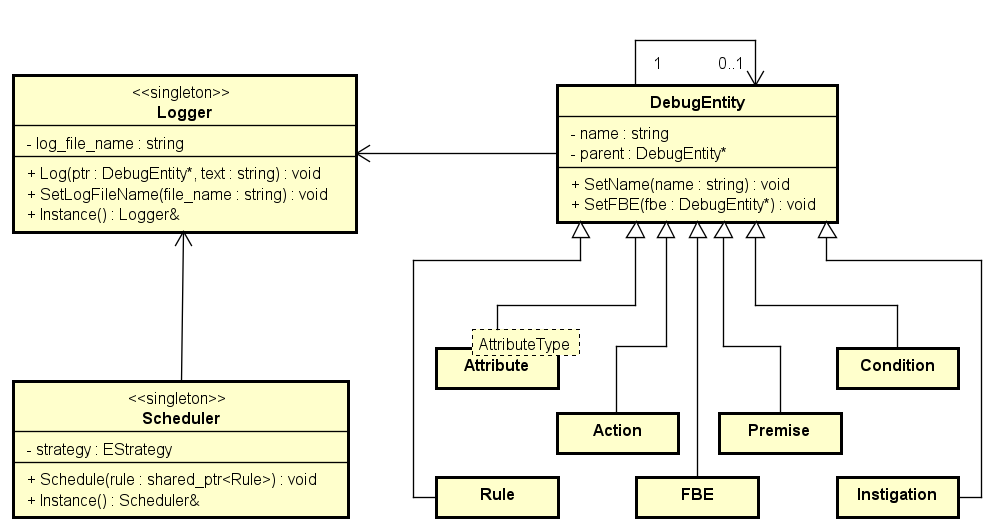
\includegraphics[width=\textwidth]{../figures/logger_class.png}
    \smallskip
    \caption*{Fonte: Autoria própria}
    \label{fig:class_fw4_log}
\end{figure}

Como a linguagem C++, ao contrário de linguagens como \textit{Python} e
\textit{JavaScript}, ainda não suporta mecanismos de reflexão de código, que
permitiriam acessar os nomes das variáveis, é necessária a criação de entidades
para armazenar estas propriedades. A classe \textit{DebugEntity} é utilizada
para este fim, contendo o nome e um ponteiro para o \textit{FBE}, caso exista,
que contém a entidade. Todas as classes das entidades do PON derivam dessa
classe \textit{DebugEntity}.

\FloatBarrier

A classe \textit{Logger} é a entidade responsável pelos registros em si,
realizando operações de escrita nos arquivos. Esta classe é implementada como um
\textit{singleton}, facilitando o seu acesso por todas as outras entidades do
código. Além das entidades do tipo \textit{DebugEntity}, a classe
\textit{Scheduler} também usa a classe \textit{Logger} para registrar a execução
das \textit{Rules}.

Para permitir a utilização desse mecanismo de \textit{log} com nomes legíveis
para o desenvolvedor foram criados uma série de \textit{builders}. Esses
\textit{builders} seguem a mesma estrutura dos \textit{builders} já apresentados
na Seção \ref{sec:builders}, com a adição de parâmetros para o nome e ponteiro
para o \textit{FBE}, conforme mostrado no Código \ref{cod:debug_builder} no
\textit{builder} da \textit{Condition}.

\lstinputlisting[language=C++, linerange={80-86}, float=htb, caption = {\textit{Builder}
            com propriedades de \textit{debug} do \textit{Framework} PON C++
            4.0}, source = {Autoria própria}, label ={cod:debug_builder}]
            {../code/Cpp-Framework-4_0/include/libnop/condition.h}

De modo a exemplificar esta utilização, a estrutura \textit{Test} e sua
respectiva implementação com o \textit{Framework} PON C++ 4.0 são apresentadas
no Código \ref{cod:debug_test}, na qual um FBE simples é inicializado nomeando
os seus membros, assim como nomeando o próprio \textit{FBE}. Um trecho de
\textit{log} resultante da utilização dessa estrutura é apresentado na Tabela
\ref{fig:log_fw4}. Nesse trecho podem ser observados os registros de mudança de
valor dos \textit{Attributes}, nas linhas 1 e 3, até a aprovação e execução da
\textit{Rule} pelo escalonador, nas linhas 7 e 8.

\begin{lstlisting}[language=C++, float=htb,
    caption = {Exemplo de
    \textit{FBE} com nomes do \textit{Framework} PON C++ 4.0},
    source = {Autoria própria},
    label = {cod:debug_test}]
/*
fbe Test
    public integer at1 = -1
    public integer at2 = -2
    public integer atExecutionCounter = 0
    private method mt
        attribution
            this.atExecutionCounter = this.atExecutionCounter + 1
        end_attribution
    end_method
    rule rlTest
        condition
            premise pr1
                this.at1 == this.at2
            end_premise
        end_condition
        action sequential
            instigation sequential
                call this.mt()
            end_instigation
        end_action
    end_rule
end_fbe
*/
struct Test : NOP::FBE
{
    explicit Test(const std::string_view name) : FBE(name) {}
    // Essa é a parte relativa a definição do FBE
    // Aqui se declaram e inicializam os Attributes
    NOP::SharedAttribute<int> at1 =
        NOP::BuildAttributeNamed("at1", this, -1);
    NOP::SharedAttribute<int> at2 =
        NOP::BuildAttributeNamed("at2", this, -2);
    NOP::SharedAttribute<int> atExecutionCounter =
        NOP::BuildAttribute(0);
    // Aqui se define o Method utilizando uma expressão lambda
    NOP::Method mt = METHOD( 
        atExecutionCounter.SetValue(executionCounter.GetValue()+1);
        );

    // Essa é a parte relativa a definição da Rule agregada ao FBE
    // com a definição das respectivas Premise, Condition, Action
    // e Instigation que a compõe
    NOP::SharedPremise pr1 =
        NOP::BuildPremiseNamed("pr1", this, at1, at2, NOP::Equal());
    NOP::SharedCondition cn1 =
        NOP::BuildConditionNamed("cn1", this, CONDITION(*pr1), pr1);        
    NOP::SharedInstigation in1 =
        NOP::BuildInstigationNamed("in1", this, mt);
    NOP::SharedAction ac1 = 
        NOP::BuildActionNamed("ac1", this, in1);

    NOP::SharedRule rl1 = NOP::BuildRuleNamed("rl1", this, cn1, ac1);
};
\end{lstlisting}

\FloatBarrier

Como esse mecanismo de \textit{log} pode ser computacionalmente bastante
custoso, aumentando os tempos de execução devido ao tempo gasto escrevendo em
arquivos, assim como aumentando o consumo de memória das entidades para
armazenar os nomes das mesmas, o \textit{Framework} PON C++ 4.0 é construído de
forma a possibilitar habilitar ou desabilitar a utilização dos \textit{logs}.
Isso é feito por meio de uma opção de compilação \textit{LIBNOP\_LOG\_ENABLE}
que pode ser configurada pelo desenvolvedor de acordo com a sua necessidade.
Esta e outras opções de compilação são detalhadas na seção seguinte.

\begin{table}[!htb]
    \begin{lstlisting}[numbers=left,
    stepnumber=1,frame=lines]
[2021-03-27 18:40:21.494] [NOP] [info] TestFBE - at1: Value changed to 1
[2021-03-27 18:40:21.494] [NOP] [info] TestFBE - pr1: Disapproved
[2021-03-27 18:40:21.494] [NOP] [info] TestFBE - at2: Value changed to 1
[2021-03-27 18:40:21.494] [NOP] [info] TestFBE - pr1: Approved
[2021-03-27 18:40:21.494] [NOP] [info] TestFBE - cn1: Approved
[2021-03-27 18:40:21.494] [NOP] [info] TestFBE - rl1: Scheduled
[2021-03-27 18:40:21.494] [NOP] [info] TestFBE - rl1: Approved
[2021-03-27 18:40:21.494] [NOP] [info] TestFBE - rl1: Executed by scheduler
[2021-03-27 18:40:21.494] [NOP] [info] TestFBE - ac1: Activated
[2021-03-27 18:40:21.494] [NOP] [info] TestFBE - in1: Instigated
\end{lstlisting}
    \caption{Exemplo de \textit{logs} do \textit{Framework} PON C++ 4.0}
    \caption*{Fonte: Autoria própria}
    \label{fig:log_fw4}
\end{table}

Ainda, para a implementação deste mecanismo é utilizada a biblioteca
spdlog\footnote{Código fonte disponível em
\url{https://github.com/gabime/spdlog}}. Esta é uma biblioteca de alto
desempenho para \textit{logs} em linguagem de programação C++. Além de facilitar
o desenvolvimento, o uso dessa biblioteca garante o funcionamento correto do
mecanismo de \textit{logs} mesmo para a execução com paralelismo, sem ocorrer
sobreposição indevida das linhas de \textit{log}, pois a biblioteca apresenta
mecanismos de controle que gerenciam a escrita dos \textit{logs}.

\section{Opções de compilação}

De modo a permitir ao desenvolvedor obter o melhor desempenho possível com o
\textit{Framework} PON C++ 4.0, alguns recursos podem ser desabilitados. Esses
recursos são o mecanismo de \textit{logs} e o escalonador. Ambos esses recursos,
apesar de úteis, aumentam os tempos de execução do \textit{software} em
\textit{Framework} PON C++ 4.0, sendo ambos desabilitados por padrão. Dito isto,
é importante ressaltar que a execução com o escalonador desabilitado apresenta o
mesmo comportamento da estratégia \textit{NO\_ONE} do \textit{Framework} PON C++
2.0.

O controle dessas opções pode ser feito por meio de definições no código. O
controle por meio de definições de código é simples, e pode ser feito inserindo
\textit{\#define LINBOP\_SCHEDULER\_ENABLE} e/ou \textit{\#define
LINBOP\_LOGGER\_ENABLE} antes de incluir os arquivos do \textit{framework},
conforme exemplificado no Código \ref{cod:defines}.

Ademais, um guia em inglês com instruções detalhadas de uso do
\textit{Framework} PON C++ 4.0, desenvolvido com o propósito de facilitar o uso
por novos desenvolvedores, é disponibilizado no \nameref{ch:manual}. Esse manual
apresenta exemplos de uso das entidades do PON, assim como instruções de
compilação\footnote{Além do manual também foi realizado um treinamento virtual
de utilização do \textit{Framework} PON C++ 4.0 que foi gravado e será
posteriormente disponibilizado na forma de vídeo}.

\begin{lstlisting}[language=C++, float=htb,
    caption = {Uso de defines do \textit{Framework} PON C++ 4.0},
    source = {Autoria própria},
    label = {cod:defines}]
#define LIBNOP_SCHEDULER_ENABLE
#define LINBOP_LOGGER_ENABLE
#include "libnop/framework.h"
\end{lstlisting}

\section{Testes unitários e de integração}\label{sec:unit_test}

A partir da implementação de todas as funcionalidades do \textit{Framework} PON
C++ 4.0, que foram apresentadas ao longo deste capítulo, foi construído um
conjunto de testes capaz de validar as funcionalidades do \textit{framework},
como a execução correta do mecanismo de notificações, bem como a aprovação de
\textit{Premises}, \textit{Conditions} e \textit{Rules} conforme o esperado em
dados contextos.

Foram desenvolvidos 38 testes englobando todas as funcionalidades do
\textit{framework}. A cada modificação feita no código, os testes são novamente
executados para se garantir que nenhuma funcionalidade que já havia sido
previamente implementada tenha sido degradada. No Código
\ref{cod:test_case_rule}, mais precisamente, é apresentado um desses testes
contemplando todas as unidades do \textit{framework} sob a forma de um teste de
integração. O conjunto completo de testes do \textit{Framework} PON C++ 4.0 está
disponível para consulta no \nameref{ap:testes}.

\begin{lstlisting}[language=C++, caption = {Caso de teste do \textit{Framework} PON C++
4.0}, source = {Autoria própria}, label ={cod:test_case_rule}]
TEST(Complete, Basic)
{
    // Criação dos Attributes
    NOP::SharedAttribute<int> at1 = NOP::BuildAttribute(-1);
    NOP::SharedAttribute<int> at2 = NOP::BuildAttribute(1);

    // Criação da Premise
    NOP::SharedPremise pr1 = NOP::BuildPremise(at1, at2, NOP::Equal());

    // Criação da Condition
    NOP::SharedCondition cn1 = NOP::BuildCondition<NOP::Single>(pr1);

    // Contador utilizado para verificar execução do método
    std::atomic<int> executionCounter{0};

    // Criação da Action com Instigation e Method criadas de forma conjunta
    NOP::SharedAction ac1 = NOP::BuildAction(
      NOP::BuildInstigation(
        METHOD(executionCounter++;)));

    // Criação da Rule
    NOP::SharedRule rl1 = NOP::BuildRule(cn1, ac1);
    // Valida estados iniciais das entidades
    EXPECT_FALSE(pr1->Approved());
    EXPECT_FALSE(cn1->Approved());
    EXPECT_FALSE(rl1->Approved());

    // Altera valor do Attribute para causar aprovação da Rule
    at1->SetValue(1);
    // Valida novos estados das entidades
    EXPECT_TRUE(pr1->Approved());
    EXPECT_TRUE(cn1->Approved());
    EXPECT_TRUE(rl1->Approved());
    // Valida execução do método por meio do contador
    EXPECT_EQ(executionCounter, 1);
}
\end{lstlisting}

Da mesma forma os Códigos \ref{cod:test_pr} e \ref{cod:test_cn} mostram,
respectivamente os casos de teste para a validação de uma \textit{Premise} e uma
\textit{Condition}. Esses são testes de unidades, mais elementares que o teste
do Código \ref{cod:test_case_rule}, que permitem uma maior granularidade no
nível dos testes, facilitando encontrar os erros em caso de falha nos testes,
pois se torna possível observar em qual unidade elementar do \textit{framework}
ocorrem problemas.

\begin{lstlisting}[caption = {Caso de teste para \textit{Premise} do \textit{Framework} PON C++ 4.0},
source = {Autoria própria}, float=htb, language=C++,
label = {cod:test_pr},
]
/*
public integer at1 = -1
public integer at2 = -2

premise prIsActivated
    this.at1 == this.at2
end_premise
*/
TEST(Premise, Simple)
{
    // Inicialização das unidades
    NOP::SharedAttribute<int> at1 = NOP::BuildAttribute<int>(-1);
    NOP::SharedAttribute<int> at2 = NOP::BuildAttribute<int>(-2);
    NOP::SharedPremise pr1 = NOP::BuildPremise(at1, at2, NOP::Equal());

    // Validação dos testes
    EXPECT_FALSE(pr1->Approved());
    at1->SetValue(1);
    EXPECT_FALSE(pr1->Approved());
    at2->SetValue(1);
    EXPECT_TRUE(pr1->Approved());
}
\end{lstlisting}

\begin{lstlisting}[caption = {Caso de teste para \textit{Condition} do \textit{Framework} PON C++ 4.0},
source = {Autoria própria}, float=htb, language=C++,
label = {cod:test_cn},
]
/*
public integer at1 = -1
public integer at2 = -2

condition
    premise prIsActivated
        this.at1 == this.at2
    end_premise
end_condition
*/
TEST(Condition, Conjunction)
{
    // Inicialização das unidades
    NOP::SharedAttribute<int> at1 = NOP::BuildAttribute<int>(-1);
    NOP::SharedAttribute<int> at2 = NOP::BuildAttribute<int>(-1);
    NOP::SharedPremise pr1 = NOP::BuildPremise(at1, 1, NOP::Equal());
    NOP::SharedPremise pr2 = NOP::BuildPremise(at2, 2, NOP::Equal());
    NOP::SharedCondition cn1 = NOP::BuildCondition<NOP::Conjuction>(pr1, pr2);

    // Validação dos testes
    EXPECT_FALSE(cn1->Approved());
    at1->SetValue(1);
    EXPECT_FALSE(cn1->Approved());
    at2->SetValue(2);
    EXPECT_TRUE(cn1->Approved());
}
\end{lstlisting}

\FloatBarrier

A Figura \ref{fig:graph_tests} mostra o relatório gerado com a execução de todos
os testes utilizando o \textit{framework} Google Test. Esse relatório foi obtido
por meio da integração da ferramenta Visual Studio 2019, que detecta
automaticamente os casos de testes escritos com o Google Test e consegue listar
os mesmos nesta interface gráfica. Nesta figura é possível observar que todos os
testes foram aprovados e que a execução levou menos de 1 segundo. 

\begin{figure}[!htb]
\centering
\caption{Relatório dos testes do \textit{Framework} PON C++ 4.0}
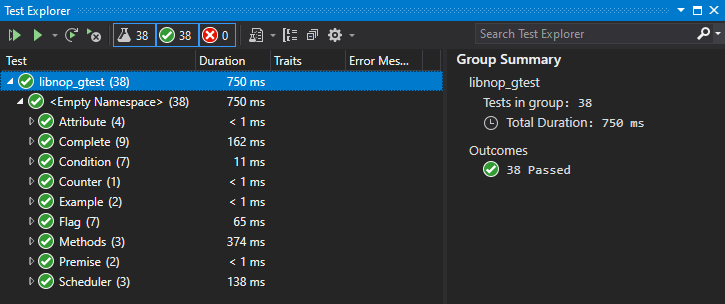
\includegraphics[width=\textwidth]{../figures/gtest_020421.png}
\smallskip
\caption*{Fonte: Autoria própria}
\label{fig:graph_tests}
\end{figure}

%Da mesma forma que foram construídos testes unitários, também foram construídos
%testes de desempenho. Nestes testes, o objetivo é realizar a construção de
%aplicações utilizando o \textit{Framework} PON C++ 4.0 que permitam avaliar o
%seu desempenho por meio do tempo de execução e consumo de memória. Esses testes
%são relatados na seção seguinte.

\section{Reflexões sobre o \textit{Framework} PON C++ 4.0}\label{sec:dev_reflex}

Dado o desenvolvimento do \textit{Framework} PON C++ 4.0, a Tabela
\ref{tab:obj_fw4_atingidos} reapresenta os objetivos propostos para o
desenvolvimento do mesmo, ressaltando que todos foram atingidos em plenitude,
conforme apresentado ao longo de todo este capítulo. Ademais, nesta seção são
feitas reflexões sobre como esses objetivos foram alcançados.

\begin{table}[!htb]
\centering
\caption{Objetivos atingidos pelo \textit{Framework} PON C++ 4.0}
\smallskip
\begin{tabularx}{\textwidth}{|l|X|l|}\hline
    Objetivo & Proposta & Atingido  \\\hline\hline
    Adicionar a flexibilidade de tipos & \textit{Attribute} com tipo \textit{template} & Sim \\ \hline
    Adicionar flexibilidade algorítmica & \textit{Condition} com expressões \textit{lambda} & Sim \\ \hline
    Reduzir a verbosidade da utilização & \textit{Builders} com \textit{variadic templates} & Sim \\ \hline
    Permitir execução com paralelismo & Notificações com políticas de execução & Sim \\ \hline
    \end{tabularx}
    \caption*{Fonte: Autoria própria}
    \label{tab:obj_fw4_atingidos}
\end{table}

A aplicação da programação genérica, por meio do uso de \textit{templates}
permitiu adicionar a flexibilidade de tipos aos \textit{Attributes},
possibilitando o uso de \textit{Attributes} com tipos definidos pelo
desenvolvedor. Ainda, tal flexibilização permitiu simplificar o código do
\textit{framework}, quando comparado ao \textit{Framework} PON C++ 2.0, por
eliminar as instâncias de código repetido que seriam necessárias para
implementar as especializações de cada tipo. 

A flexibilidade algorítmica, por sua vez, é alcançada com a criação do conceito
de \textit{Condition} flexível, possibilitado pelo uso de expressões
\textit{lambda} para a definição da operação booleana entre as
\textit{Premises}. Naturalmante, como esse é um conceito novo introduzido pelo
\textit{Framework} PON C++ 4.0, ainda não é possível de ser representado com a
NOPL.

Entretanto, a adição do conceito de \textit{Condition} flexível, apesar de
facilitar a programação em alto nível, dificulta a implementação do conceito de
impertinência. A implementação do conceito de impertinência depende da entidade
\textit{Condition} ser capaz de avaliar o número de \textit{Premises} que devam
mudar de estado para poder ser aprovada, de modo a ser capaz de remover a
impertinência quando necessário. A adição da flexibilidade algorítmica,
implementada através de expressões \textit{lambda} no \textit{Framework} PON C++
4.0, abstrai o número de premissas e a operação realizada entre elas, de modo
que a classe \textit{Condition} se torna incapaz de avaliar a impertinência das
entidades.

Deste modo, o conceito de impertinência fica de fora do escopo da implementação
do \textit{Framework} PON C++ 4.0 neste trabalho, porém ela pode ser
implementada em trabalhos futuros. A implementação de impertinência no
\textit{Framework} PON C++ 4.0 pode ser feita com a implemetação de classes que
realizem o tratamento de \textit{Conditions} apenas com disjunções ou
conjunções, não permitindo a expressão de \textit{Condition} com flexibilidade
algorítmica. Essas novas classes naturalmente herdariam da classe
\textit{Condition} e implementariam a lógica específica para o tratamento de
impertinência.

A redução da verbosidade da utilização é dada principalmente com a implementação
dos \textit{Builder}, que utilizando os recursos avançados da linguagem de
programação C++ dita moderna, como \textit{variadic templates} e \textit{fold
expression}, permitiu a criação de interfaces bastante simples de utilizar, mas
que também apresentam a flexibilidade necessária para o uso. Desta forma, como
fica evidente ao longo dos diversos códigos apresentados neste capítulo,
\textit{Framework} PON C++ 4.0 permite uma estrutura de declaração de suas
entidades de forma muito similar a estrutura da NOPL, contribuindo assim com a
facilitação da programação em alto nível, de modo similar ao almejado pelo
prototipal JuNOC++.

A questão do paralelismo é tratada de forma bastante transparente,
visto que com a adição de recursos como as políticas de execução foi possível a
implementação de código altamente paralelizável sem ser necessária a adição de
mecanismos complexos de controle. A complexidade referente ao paralelismo é
tratada justamente por esses recursos da linguagem, não sendo necessário
reimplementar no \textit{framework}.

O paralelismo é, de fato, implementado de duas principais maneiras, utilizando
as notificações paralelizadas por meios das políticas de execução em si, e
também por meio do uso de \textit{Methods} paralelizáveis. O \textit{framework}
apresenta uma maneira padrão de se criar \textit{Methods} paralelizáveis (pelo
uso da \textit{macro} \textit{ASYNC\_METHOD}), porém o desenvolvedor também é
livre para implementar seus próprios mecanismos de paralelização caso seja
necessário, devido à flexibilidade dada pelo uso das expressões \textit{lambda}.

Além disso, o conjunto de testes unitários e de integração desenvolvidos à luz
do método TDD se prova essencial para avaliar o funcionamento das entidades
desenvolvidas no \textit{Framework} PON C++ 4.0. Entretanto, a aplicação diverge
um pouco do método proposto por \citeonline{msc_Kossoski_2015}, devido ao método
ser proposto para o teste de aplicações, e não de frameworks. Dessa forma, não
há a existência de casos de uso em nível de aplicação, como utilizado no método
de \citeonline{msc_Kossoski_2015} para levantamento dos casos de teste. Ainda
assim, se aproveitam os conceitos de testes comuns às entidades do PON, como as
classes de equivalência para testes de \textit{Premises}. Apesar disso, o
\textit{Framework} PON C++ 4.0 também evolui sobre o método proposto ao aplicar
o uso de \textit{frameworks} de teste para automatizar o processo de testes.

Por fim, também é importante abordar a questão do desempenho, pois a construção
do \textit{Framework} PON C++ 4.0 utiliza diversos recursos da STL em sua
composição, como \textit{std::vector}, \textit{std::functions},
\textit{std::unique\_ptr} e \textit{std::shared\_ptr}. A utilização destas
estruturas pode incorrer em um aumento do tempo de execução de programas devido
ao custo computacional da utilização destas estruturas.

Esse custo de desempenho poderia ficar aparente principalmente quando comparado
ao \textit{Framework} PON C++ 2.0, que não utiliza estas entidades
computacionais potencialmente custosas, ao optar por uma implementação
utilizando estruturas de dados dedicadas, justamente com o objetivo de se obter
um melhor desempenho com um menor tempo de execução \cite{msc_valenca_2012}.

Ainda assim, o uso eficiente dos recursos da STL possibilita uma melhor
estruturação algorítmica do código, o que por sua vez pode melhorar o desempenho
ao diminuir os tempos de execução. Essa melhor estruturação algorítmica
possibilita um melhor aproveitamento do recurso de compartilhamento de
entidades, reduzindo o número de entidades como \textit{Premises} e
\textit{Conditions} necessárias, o que por sua vez também reduz número de
notificações geradas no sistema.

De modo a ilustrar os benefícios dessa melhor estruturação algorítmica com o
\textit{Framework} PON C++ 4.0, o Código \ref{cod:excomplex} mostra como é
complicada a construção da \textit{Condition} \textit{mainCondition} que faz a
combinação de diversas \textit{Premises} e exigindo o uso de duas
\textit{SubConditions}, enquanto o Código \ref{cod:exsimple} simplifica essa
mesma construção por meio do uso das \textit{Conditions} com flexibilidade
algorítmica. Essa melhoria permite reduzir o número de entidades necessárias
para a construção do código, passando de quatro \textit{Premises} e três
\textit{Conditions} para apenas três \textit{Premises} e uma única
\textit{Condition}, com isso reduzindo o número de notificações necessárias para
aprovar uma \textit{Rule} e melhorando a expressividade do código.

\begin{lstlisting}[caption = {Construção complexa de \textit{Condition} com o \textit{Framework} PON C++ 4.0},
source = {Autoria própria}, %float=htb,
label = {cod:excomplex},
]
/*
condition mainCondition
    subcondition cn1
        premise prIsNotAt1 at1 == false
        and
        premise prIsAt2 at2 == true
    end_subcondition
    or
    subcondition cn2
        premise prIsAt1 at1 == true 
        and
        premise prIsAt3 at3 == true
    end_subcondition
end_condition
*/

NOP::SharedAttribute<bool> at1 = NOP::BuildAttribute(false);
NOP::SharedAttribute<bool> at2 = NOP::BuildAttribute(false);
NOP::SharedAttribute<bool> at3 = NOP::BuildAttribute(false);
NOP::SharedPremise prIsAt1 = NOP::BuildPremise<bool>(at1, true, NOP::Equal());
NOP::SharedPremise prIsNotAt1 = NOP::BuildPremise<bool>(at1, false, NOP::Equal());
NOP::SharedPremise prIsAt2 = NOP::BuildPremise<bool>(at2, true, NOP::Equal());
NOP::SharedPremise prIsAt3 = NOP::BuildPremise<bool>(at3, true, NOP::Equal());
NOP::SharedCondition cn1 = NOP::BuildCondition<NOP::Conjunction>(prIsNotAt1, prIsAt2);
NOP::SharedCondition cn2 = NOP::BuildCondition<NOP::Conjunction>(prIsAt1, prIsAt3);
NOP::SharedCondition mainCondition = NOP::BuildCondition<NOP::Disjunction>(cn1, cn2);

\end{lstlisting}

\begin{lstlisting}[caption = {Construção simplificada de \textit{Condition} com o \textit{Framework} PON C++ 4.0},
source = {Autoria própria}, float=htb,
label = {cod:exsimple},
]
NOP::SharedAttribute<bool> at1 = NOP::BuildAttribute(false);
NOP::SharedAttribute<bool> at2 = NOP::BuildAttribute(false);
NOP::SharedAttribute<bool> at3 = NOP::BuildAttribute(false);
NOP::SharedPremise prIsAt1 = NOP::BuildPremise<bool>(at1, true, NOP::Equal());
NOP::SharedPremise prIsAt2 = NOP::BuildPremise<bool>(at2, true, NOP::Equal());
NOP::SharedPremise prIsAt3 = NOP::BuildPremise<bool>(at3, true, NOP::Equal());
NOP::SharedCondition mainCondition = NOP::BuildCondition(CONDITION(
    (!*prIsAt1 && *prIsAt2) || (*prIsAt1 && *prIsAt3) ),
    prIsAt1, prIsAt2, prIsAt3);
\end{lstlisting}

Observando os resultados atingidos pelo desenvolvimento do \textit{Framework}
PON C++ 4.0, apresentados neste Capítulo, é interessante analisar de que forma
este novo \textit{framework} avança sobre as propriedades elementares e
conceitos comparados aos outros \textit{frameworks} disponíveis. Estes conceitos
foram anteriormente introduzidos na Seção \ref{sec:conceitos_pon}. A propriedade
de distribuição do PON ainda não foi contemplada na implementação atual do
\textit{Framework} PON C++ 4.0, porém trabalhos futuros pretendem contemplar
esta propriedade em futuras melhorias no \textit{framework}. A Tabela
\ref{tab:elementares_2} resume estes resultados.

\begin{table}[!htb]
\centering
\caption{Propriedades elementares contempladas nas materializações do PON}
\smallskip
\begin{threeparttable}
\begin{tabularx}{\textwidth}{|l||*{9}{X|}}\hline
\diagbox{Potencial\\ de propriedade}{Materialização} & 
Fw. C++ Prot. & Fw. C++ 1.0 & Fw. C++ 2.0 & Fw. C++ 3.0 & \textbf{Fw. C++ 4.0} & Fw. Java /C\# & Fw. C\# IoT & Fw. Elixir & Fw. Akka \\\hline\hline
\makecell{Programação\\ em alto nível}             & \textasciitilde & \textasciitilde & $\star$ & \textasciitilde & \checkmark & \textasciitilde & \textasciitilde & \textasciitilde & \textasciitilde \\\hline
\makecell{Paralelismo\\ via desacoplamento}        & & & & \textasciitilde & \checkmark & & \checkmark & \checkmark & \checkmark \\\hline
\makecell{Distribuição\\ via desacoplamento}       & & & & & $\circ$ & & \checkmark & * & * \\\hline
\makecell{Desempenho\\ via não redundâncias}       & & & \textasciitilde & & \checkmark & \textasciitilde & & & \\\hline
\end{tabularx}
\begin{tablenotes}
  \item[\checkmark] Materializa completamente a propriedade
  \item[\textasciitilde] Materializa parcialmente a propriedade
  \item[$\star$] Materializa a propriedade por meio de ferramenta \textit{wizard} \cite{msc_valenca_2012}
  \item[*] A tecnologia de base permite a propriedade, entretanto carece de
  testes para validação
  \item[$\circ$] Trabalho subsequente proposto de Pelegrine Figueiredo detalhado na Seção
  \ref{sec:pon_dist}
\end{tablenotes}
\end{threeparttable}
\caption*{Fonte: Autoria própria}
\label{tab:elementares_2}
\end{table}

Pelo fato do \textit{Framework} PON C++ 4.0 se tratar de uma evolução sobre o
\textit{Framework} PON C++ 2.0, era de se esperar que todos os conceitos de
programação materializados no \textit{Framework} PON C++ 2.0 também se
encontrassem no \textit{Framework} PON C++ 4.0. A tabela \ref{tab:conceitos2}
apresenta os conceitos de programação materializados pelos diferentes
\textit{frameworks}, destacando o \textit{Framework} PON C++ 4.0. Em suma, no
que diz respeito aos conceitos atingidos é possível notar que o
\textit{Framework} PON C++ 4.0 apresenta os conceitos que o \textit{Framework}
PON C++ 2.0 materializava, com a exceção da impertinência estática e
\textit{Keeper}, porém também materializa o conceito de \textit{Condition}
flexível.

\begin{table}[!t]
\centering
\caption{Conceitos do PON contemplados nas materializações do paradigma - com adição do \textit{Framework}
PON C++ 4.0}
\smallskip
\begin{threeparttable}
\begin{tabularx}{\textwidth}{|l||*{9}{X|}}\hline
\diagbox{Conceito de \\Programação}{Materialização} & Fw. Prot. & Fw. C++ 1.0 &
Fw. C++ 2.0 & Fw. C++ 3.0 & \textbf{Fw. C++ 4.0} & Fw. Java /C\#& Fw. C\# IoT &
Fw. Elixir & Fw. Akka \\\hline\hline
Reatividade das entidades
&\checkmark&\checkmark&\checkmark&\checkmark&\checkmark&\checkmark&\checkmark&\checkmark&\checkmark\\\hline
Compartilhamento de entidades
&&\checkmark&\checkmark&\checkmark&\checkmark&\checkmark&\checkmark&\checkmark&\\\hline
Renotificações
&&\checkmark&\checkmark&\checkmark&\checkmark&\checkmark&&&\\\hline
Resolução de conflitos
&&\checkmark&\checkmark&\checkmark&\checkmark&\checkmark&\checkmark&&\\\hline
\textit{Master Rule} &&&\checkmark&\checkmark&\checkmark&&&&\\\hline
Impertinência estática &&&\checkmark&\checkmark&&&&&\\\hline
Impertinência dinâmica &&&&&&&\checkmark&&\\\hline
\textit{FBE Rules} &&&\checkmark&\checkmark&\checkmark&&&&\\\hline
\textit{FBE} Agregador &&&\checkmark&\checkmark&\checkmark&&&&\\\hline
\textit{Formation Rules} &&&&&&&&&\\\hline
\textit{Keeper} &&&*&&&&&&\\\hline
\textit{Condition} flexível &&&&&\checkmark&&&&\\\hline
\end{tabularx}
\begin{tablenotes}
  \item[*] Implementado sob a forma de uma adaptação no \textit{framework}
  existente, visto que altera o fluxo tradicional de execução das
  \textit{Rules} do PON \cite{muchalski_2012}
\end{tablenotes}
\end{threeparttable}
\caption*{Fonte: Autoria própria}
\label{tab:conceitos2}
\end{table}

Devido ao aumento da flexibilidade dado pela adição do conceito de
\textit{Condition} flexível é dificultada a implementação do conceito de
impertinência, conforme discutido na Seção \ref{sec:estrutura_fw4}. Ainda, um
dos objetivos da adição do conceito de impertinência é justamente melhorar o
desempenho das aplicações. Entretanto, espera-se que, apesar de não contar com a
materialização desse conceito, reduza os tempos de execução das aplicações em
PON ao permitir uma melhor eficiência na composição e compartilhamento das
entidades e também ao reduzir o número de entidades totais do código, como
demonstrado nos Códigos \ref{cod:excomplex} e \ref{cod:exsimple}. Ainda, o
conceito \textit{Keeper} também não é materializado, visto que sua implementação
altera o fluxo tradicional de execução das \textit{Rules} do PON
\cite{muchalski_2012}, podendo ser facilmente implementado com as mesmas
adaptações que foram necessárias no \textit{Framework} PON C++ 2.0. Por fim, o
conceito de \textit{Formation Rules} também não é implementado por nenhum
\textit{framework} sendo materializado apenas por meio da tecnologia LingPON,
visto que tal nível de abstração é difícil de ser implementado nas linguagens de
programação dos \textit{frameworks}, pois exige uma etapa de compilação para
interpretar a expressão destas \textit{Rules}.


Os resultados obtidos por meio da utilização do \textit{Framework} PON C++ 4.0
para o desenvolvimento de aplicações são detalhados no capítulo seguinte. Nesses
resultados é inclusive discutida a efetividade das implementações de
paralelização no \textit{Framework} PON C++ 4.0.